\documentclass[11pt,letterpaper]{article}
\usepackage[margin=.86in,top=.79in,bottom=.79in,headheight=16pt]{geometry}
\usepackage{amsmath,amssymb,graphicx,booktabs,xcolor,hyperref,fancyhdr}
\definecolor{ink}{RGB}{27,55,67}
\definecolor{teal}{RGB}{33,100,98}
\hypersetup{colorlinks=true,linkcolor=teal,urlcolor=teal,pdftitle={Intrinsic diameters of four regular solids}}
\pagestyle{fancy}\fancyhf{}\lhead{\small\sffamily Intrinsic diameters of four regular solids}\rhead{\small\sffamily Surface geometry}\cfoot{\small\thepage}
\setlength{\parindent}{0pt}\setlength{\parskip}{.43em plus .05em minus .04em}
\setlength{\abovedisplayskip}{7pt plus 2pt minus 2pt}\setlength{\belowdisplayskip}{7pt plus 2pt minus 2pt}
\setlength{\emergencystretch}{1.5em}
\newcommand{\R}{\mathbb R}\newcommand{\N}{\mathbb N}\newcommand{\Q}{\mathbb Q}
\newcommand{\1}{\mathbf 1}

\renewcommand{\labelitemi}{\(\bullet\)}
\begin{document}
\thispagestyle{plain}
{\large\sffamily\color{teal} Polyhedral geometry and constructive arithmetic}\par\medskip
{\LARGE\bfseries\color{ink} Intrinsic diameters of four regular solids}\par
{\large Farthest points from a vertex and from a freely chosen point}\par\smallskip
{\small 19 November 2026}\par\medskip
For a solid $P$ of unit edge length let $d(x,y)$ be the infimum of the lengths of all continuous rectifiable paths on $\partial P$ from $x$ to $y$. A path can cross an edge or run along it. Write $R_V=\max_y d(V,y)$ for a chosen vertex $V$, and $D=\max_{x,y}d(x,y)$. These are the two questions in the supplied cuboid reports. The origins in the following results are the centers of the solids.
\begin{center}
\renewcommand{\arraystretch}{1.35}
\begin{tabular}{@{}llll@{}}\toprule
Solid & Unique farthest point from $V$ & $R_V=D$ & Unordered pairs\\\midrule
Tetrahedron & Opposite face centroid $-V/3$ & $2/\sqrt3$ & $4$\\
Octahedron & Opposite vertex $-V$ & $\sqrt3$ & $3$\\
Icosahedron & Opposite vertex $-V$ & $\sqrt7$ & $6$\\
Dodecahedron & Opposite vertex $-V$ & $\sqrt{(17+7\sqrt5)/2}$ & $10$\\\bottomrule
\end{tabular}
\end{center}
The last column counts \emph{all} pairs attaining $D$. Thus freeing the first endpoint gives no increase for any of the four solids. Symmetry has two meanings here. Every maximizing pair lies on a rotation axis. Central inversion exchanges the two ends in the last three cases. No tetrahedral symmetry exchanges a vertex and a face centroid. For edge length $a>0$, multiply the distances and the unit-model coordinates by $a$.
\paragraph{Coordinates.} Write $\phi=(1+\sqrt5)/2$. In the order of the table, one can take
\[
 V=\frac{(1,1,1)}{2\sqrt2},\qquad
 V=\frac{(0,0,1)}{\sqrt2},\qquad
 V=\frac{(0,1,\phi)}2,\qquad
 V=-\frac{\phi}2(1,1,1).
\]
The tetrahedron consists of the four sign patterns with positive product. The octahedron has the six coordinate-axis vertices. The icosahedron has the cyclic permutations of $(0,\pm1,\pm\phi)/2$. The full dodecahedral coordinate model appears in Section~\ref{sec:dod}. The symmetry group acts transitively on the vertices in each case.
\begin{center}
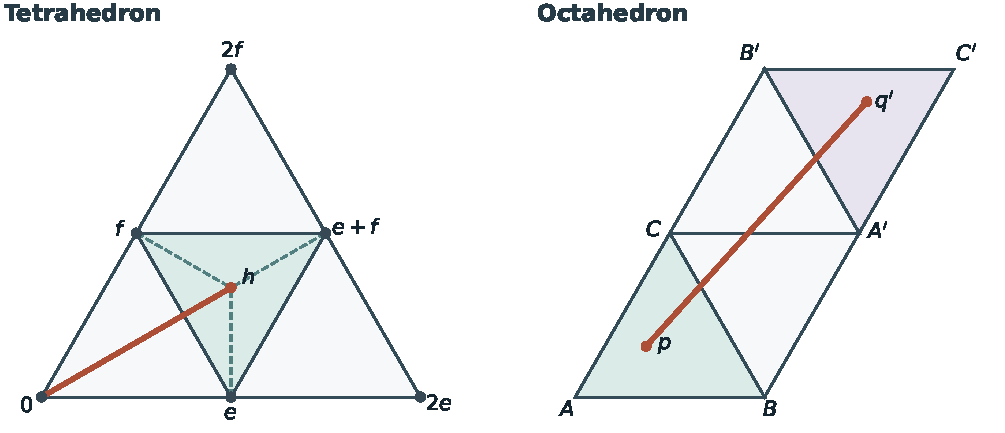
\includegraphics[width=.80\linewidth]{figures/unfoldings.pdf}\par
\small Left, the segment from a tetrahedral vertex lift to the nearest lift of the opposite face center. Right, a four-face octahedral development joining points on opposite faces.
\end{center}
\clearpage
\section{Folding and comparing surface routes}
A \emph{facewise path} is a finite list of segments, each contained in a specified closed face, with matching endpoints. An unfolding along a list of edge-adjacent faces puts the polygons in one plane by successive hinge rotations, placing consecutive interiors on opposite sides of their common edge. It preserves the length of a path following that list. To fold a straight segment back to the surface one must verify that it meets the listed hinges in order and within each closed edge. Then each intermediate subsegment is a chord of the appropriate convex face. This distinction matters in the dodecahedron. Section~\ref{sec:continuity} proves that facewise paths suffice for lower bounds even on paths with arbitrarily many edge crossings.
\paragraph{Reduction to two opposite chambers.}
Divide each polygonal face into triangles with corners a vertex, an incident edge midpoint, and the face center. Call each such closed triangle a chamber. In the octahedron, icosahedron, and dodecahedron, if $C$ is one chamber, it suffices for an upper bound to treat $C\times(-C)$. More precisely, for any $p,q$ there exist $x\in C$, $y\in-C$ and a length-nonincreasing map sending $x,y$ to $p,q$, respectively. Each endpoint is transported by a symmetry of the solid, possibly a different one at each end.
\par
Here is the folding argument. Cone each chamber from the center of the solid. Reflection in the plane of each cone wall is a symmetry, interchanging the two flags that share this wall. For example the three wall reflections exchange the two ends of an edge, the two edges of a face at the vertex, or the two faces at the edge. This follows from regularity of the flag action: the symmetry between adjacent flags fixes the other two corner rays and the origin. It thus fixes their plane and is the reflection. The mirrors of these reflections form a finite plane arrangement. They do not meet a chamber interior there: a symmetry fixing an interior point of a flag must preserve its chamber, hence the vertex, edge and face of the flag, and fixing all three corners forces identity. Thus the open chamber cones are exactly the open cells of the arrangement. In particular two adjacent cones differ in the sign of just their common wall.
\par
By one isometry move $p$ to $x\in C$ and let $q$ lie in a tagged chamber $B$. If $B\ne-C$, some facet of its cone has the interior of $-C$ on its far side. Indeed, a closed cone is the intersection of its facet halfspaces. Reflect $B$ across that wall. The number of mirror signs that differ from $-C$ decreases by one. In at most the number of mirrors this gives a gallery from $B$ to $-C$ and transports $q$ to $y$. Reverse the gallery. At every step, fold the space by reflecting the halfspace on the $-C$ side of the wall into the halfspace containing $C$. This piecewise isometry preserves the surface and fixes $x$. It takes the moving endpoint back across that wall. Such a fold is nonexpansive for Euclidean distances (the normal coordinate becomes its signed absolute value), so it is nonexpansive for path lengths. Composing with the initial inverse isometry gives the assertion. Edge and vertex endpoints allow either incident chamber.
\paragraph{Interpolation on a strip.}
Suppose paths between the corners $s_i,t_j$ of two chamber triangles use the same face list. On each hinge take the weighted mean of their crossing points with weights $w_{ij}=\lambda_i\mu_j$. These points still belong to the hinges. Join them face by face, starting at $\sum_i\lambda_i s_i$ and ending at $\sum_j\mu_j t_j$. Within each face the new segment is the weighted sum of the old displacement vectors. If the old lengths are $l_{ij}$, the new path has length at most $\sum w_{ij}l_{ij}$, hence square at most $\sum w_{ij}l_{ij}^2$. This proves a uniform upper bound from nine paths, including for a nonconvex development. When two strips are available, the shorter squared length is bounded above by their average.
\section{The tetrahedron: a vertex and the opposite face centre}
Write $e=(1,0)$ and $f=(1/2,\sqrt3/2)$ and put $L=\mathbb Ze+\mathbb Zf$. Mark the vertices of the unit equilateral triangular tiling by the four classes of $L/2L$. Each triangle has three distinct marks. Map it isometrically to the face of the unit tetrahedron with those three vertex labels. The maps agree along edges. The resulting folding identifies precisely
\[
 u\sim u+2\ell\sim -u+2\ell\qquad(\ell\in L).
\]
Indeed a fundamental parallelogram of $2L$ has eight unit triangles. Opposite triangles modulo $2L$ under $u\mapsto-u$ give four pairs, one for each possible missing mark. On interiors there is one image per pair. The sides are glued according to their two endpoint marks, and the four lattice marks give the four tetrahedron vertices. This verifies the identification also on the boundary of a triangle.

Put $\delta(w)=\min_{k\in2L}|w-k|$. For two lifts $u,v$ the surface distance is
\[
 d([u],[v])=\min\{\delta(u-v),\delta(u+v)\}.
\]
Each minimizing planar segment folds to a path of the same length. For the reverse bound, with $u$ fixed the right side is the planar distance from $v$ to the orbit of $u$. It is invariant under the identifications and is $1$-Lipschitz on each face, by the triangle inequality. It is consequently $1$-Lipschitz along surface paths, and has value zero at $[u]$. Equivalently one can sum its changes along any broken line crossing faces. Only finitely many lattice shifts are necessary when the lifts are in a bounded fundamental parallelogram: in the coordinates $e,f$, $|me+nf|^2=m^2+mn+n^2\ge(m^2+n^2)/2$.

The large triangles of the tiling on $2L$ have side $2$. In one such triangle the region closest to a given vertex is the quadrilateral with corners the vertex, the two adjacent edge midpoints, and the triangle centre. Their respective distances to the vertex are $0,1,1,2/\sqrt3$. Squared distance is convex. Hence every point has $\delta\le 2/\sqrt3$, with equality only at the large triangle centres. At a centre the three vertices are nearest: for the representative $h=2(e+f)/3$ this follows directly by minimizing $|h-2me-2nf|^2$; any other possibility of distance at most $2/\sqrt3$ would have $m,n\in\{0,1\}$ by the displayed quadratic bound, and the fourth choice $(1,1)$ is further away. An alternative integer certificate for this last lower bound is
\[
 Q(1-3m,1-3n)=3+9(m^2+mn+n^2-m-n),\qquad Q(x,y)=x^2+xy+y^2 .
\]
A nonnegative integer congruent to three modulo nine is at least three, and the squared distance under consideration is $4Q(1-3m,1-3n)/9$. All centres have residues $h$ or $-h$ modulo $2L$.

For the fixed vertex $[0]$ the two centre classes identify, giving a unique farthest point $[h]$. The unit triangle with vertices $e,f,e+f$ has its centre there and has exactly the three marks other than $[0]$. Thus $Y$ is the centroid of the opposite face. For a concrete embedding take $X=(1,1,1)/(2\sqrt2)$ and the other vertices obtained by changing two signs. Then $Y=-X/3$. The free and fixed maxima both equal $2/\sqrt3$. In fact if the free maximum is attained, $u-v$ and $u+v$ must both represent holes $\pm h$ modulo $2L$. Equal hole residues give $2v\in 2L$, so $[v]$ is a vertex. Opposite residues give $2u\in2L$, so $[u]$ is a vertex. The unique fixed-vertex result classifies every maximizing pair.

\section{The octahedron: six strips and a constant average}
Use the unit-edge realization with vertices $\pm e_i/\sqrt2$, where $e_i$ are the standard coordinate vectors in $\mathbb R^3$. Faces correspond to choices of three signs. By symmetry a source $p$ belongs to the positive face $ABC$. For any target $q$ put $q'=-(|q_1|,|q_2|,|q_3|)$ on the all-negative face. Whenever $q_i>0$, fold the $i$th coordinate to its absolute value. These folds fix $p$, send $q'$ to $q$ and preserve the surface equation $\sum |x_i|=1/\sqrt2$. They are Euclidean $1$-Lipschitz and so do not increase surface path lengths. Faces, with an assigned sign also on a zero coordinate, give the same construction without any sign test on a real coordinate. Thus it suffices to bound $d(p,q')$.

Choose any permutation of the axes and cross the three sign walls in that order. For order $A,B,C$, use coordinates in the planar triangular basis $(e,f)$ above. The positive face has vertices $(0,0),(1,0),(0,1)$ respectively. The successive reflected vertices $A',B',C'$ are $(1,1),(0,2),(1,2)$. Each new vertex is the sum of the two shared endpoints minus the vertex it replaces. The four triangles tile the convex parallelogram $[0,1]\times[0,2]$ in these coordinates. Thus the segment between \emph{any} barycentric points of the first and last triangle folds to a legal surface path. The squared distances between its possible endpoint vertices form the following matrix, rows in order $A,B,C$ and columns in order $A',B',C'$:
\[
 M=\begin{pmatrix}3&4&7\\1&3&4\\1&1&3\end{pmatrix}.
\]
Let $p$ and $q'$ have probability vectors of barycentric weights $a_i$ and $b_i$ in matched axis order. For a strip $s$, call its developed endpoints $P_s,Q_s$. The usual variance identity, applied to independent choices of the endpoint vertices with these weights, gives
\[
 |P_s-Q_s|^2=\sum_{i,j}a_i b_j M^s_{ij}
 -\sum_{i<j}a_i a_j-\sum_{i<j}b_i b_j.
\]
Here all the intervertex distances \emph{within} each endpoint triangle equal one. As the six orders vary, their matrices $M^s$ simultaneously permute the rows and columns of $M$. Their average has every entry equal to $3$: each diagonal entry is $3$, and the sum of the off-diagonal entries is $18$. Taking a shortest one of these six paths yields the stronger bound
\[
 d(p,q)^2\le 3-\sum_{i<j}a_i a_j-\sum_{i<j}b_i b_j.
\]
In particular equality at $3$ requires each vector of weights to be supported on a single vertex. This deduction also has a direct apartness version: if the sum of the three products vanishes, choose an index with weight at least $1/4$ by a fixed coarse approximation, so each other weight is zero.

Finally fix the poles $X=e_3/\sqrt2$ and $Y=-X$. Equatorial edges lie in $z=0$. Define a scalar height $H$ by affine interpolation on faces, giving values $\sqrt3/2$ at $X$, $0$ on the equator, and $-\sqrt3/2$ at $Y$. Each triangle has altitude $\sqrt3/2$, so its affine gradient has length one. Therefore every surface path joining the poles has length at least $\sqrt3$, the change in $H$. Unfolding two faces sharing an equatorial edge, their two altitudes form a straight path of that length. Any two other distinct vertices are joined by a unit edge. The fixed and free maxima are both $\sqrt3$, and the three pairs of opposite vertices are precisely all unordered diametral pairs.

\section{Icosahedron: two parallelograms and a distance bound}

Take the edge length to be one. Put $N$ at a vertex and $S=-N$ at the
opposite vertex, with the origin at the center. Label the intervening
vertex rings $A_i,B_i$ in cyclic order, $i\in\mathbb Z/5\mathbb Z$, so
that the twenty faces are
\[
 T_i=(N,A_i,A_{i+1}),\quad U_i=(A_i,A_{i+1},B_i),\quad
 V_i=(A_i,B_{i-1},B_i),\quad W_i=(S,B_i,B_{i+1}).
\]
With this labeling $-A_i=B_{i+2}$. For example, in the projection along
$NS$, the $B$-ring is offset from the $A$-ring by half a step. Use a
triangular-lattice basis of unit vectors at angle $60^\circ$ and put
$Q(u,v)=u^2+uv+v^2$.

\paragraph{A lower bound on the length of every surface path.}
We construct a scalar function $h$ which changes by at most the length
traversed. On each indicated part of a face take $h=\sqrt Q$ after the
isometric placement in the table. In each of the last two rows, $M$ is
the midpoint of the edge joining the two $B$ vertices. Apply the same
placement to both halves of the face, taking $B$ to be the vertex of
the respective half.
\[
\begin{array}{c|c|ccc}
\text{face}&\text{vertices in order}&\multicolumn{3}{c}{\text{planar coordinates}}\\ \hline
T_i&N,A_i,A_{i+1}&(0,0)&(1,0)&(0,1)\\
U_i&A_i,A_{i+1},B_i&(1,0)&(0,1)&(1,1)\\
V_i\text{, half}& A_i,B,M&(1,0)&(1,1)&(3/2,1/2)\\
W_i\text{, half}& S,B,M&(2,1)&(1,1)&(3/2,1/2)
\end{array}
\]
For clarity, the values of $h^2$ at $N,A,B,S$ are $0,1,3,7$.
Its midpoint values on edges of types $NA,AA,AB,BB,BS$ are
$1/4,3/4,7/4,13/4,19/4$, respectively. Along a shared segment of
length $l$, the squared functions from the two sides, parameterized on
$[0,1]$, have the same quadratic coefficient $l^2$. Their agreement
at the endpoints proves agreement along the entire segment. On each
piece the reverse triangle inequality for the planar norm gives the
required Lipschitz bound. Adding it along a broken path and applying
the surface-path correspondence gives
\[
 d(N,S)\ \geq\ h(S)-h(N)=\sqrt7 .
\]

\paragraph{Uniform upper bound.}
Use the chamber-folding lemma with $C$ having corners $N$, the midpoint
of $NA_0$, and the center of $T_0$. It suffices to bound distances for
$x\in C$ and $y\in -C$. The antipodal chamber lies in $W_2$. Two
six-face routes from $T_0$ to $W_2$ are
\[
 T_0,T_4,T_3,U_3,V_3,W_2,\qquad
 T_0,U_0,V_1,W_0,W_1,W_2 .
\]
Place $T_0$ as in the first row of the preceding table. To check each
development by hand, across an edge with ends $a,b$ the new third
vertex is $a+b-c$, where $c$ was the previous third vertex. The first
route fills the parallelogram $0\le u\le1$, $-2\le u+v\le1$. The second
fills $0\le u\le1$, $0\le v\le3$. Convexity makes every segment from
the starting chamber to the respective terminal chamber a legal
surface route, including the boundary by direct folding. In vertex,
edge-midpoint, face-center order, the corner lists are
\[
\begin{array}{c|ccc}
 C &(0,0)&(1/2,0)&(1/3,1/3)\\
 -C\text{ in route 1}&(1,-3)&(1/2,-5/2)&(2/3,-7/3)\\
 -C\text{ in route 2}&(1,2)&(1/2,5/2)&(2/3,8/3).
\end{array}
\]
\begin{figure}[htbp]
\centering
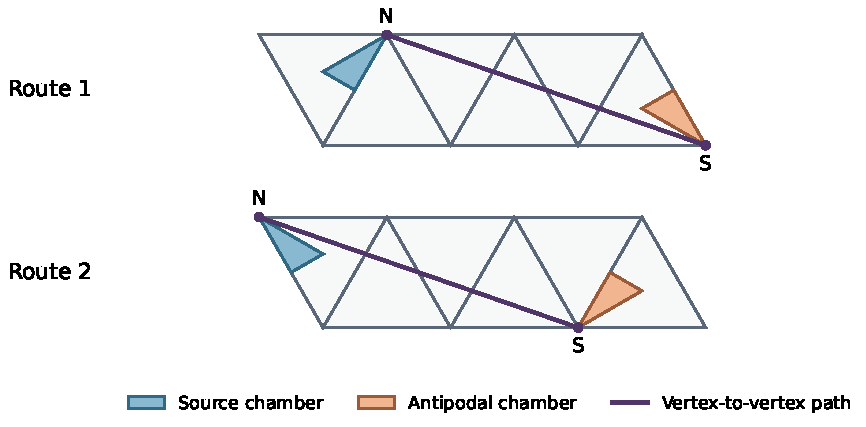
\includegraphics[width=.78\linewidth]{figures/ico_strips.pdf}
\caption{Two developments of the icosahedral surface. Each of the two
shaded triangles is a flag chamber. The displayed segments join
opposite vertices; every choice of a point in each shaded chamber also
gives a valid segment in the corresponding parallelogram.}
\end{figure}
Let $L_1,L_2$ be the two developed segment lengths. The matrix of
$(L_1^2+L_2^2)/2$ on the nine corner pairs, with rows indexed by $C$,
is
\[
 \begin{pmatrix}
 7&13/2&41/6\\ 13/2&25/4&19/3\\ 41/6&19/3&19/3
 \end{pmatrix}.
\]
For barycentric coordinates $\lambda_i$ and $\mu_j$ in the two
chambers, each developed displacement is the weighted sum of the
nine corner displacements with weights $\lambda_i\mu_j$. Convexity
of $Q$ bounds the average by the corresponding weighted sum of the
displayed matrix. The shorter route consequently has squared length at
most $7$. The gap from $7$ in every entry except the upper left is at
least $1/6$, so the same proof gives
\[
 d(x,y)^2\leq 7-\tfrac16(1-\lambda_1\mu_1),
\]
where the subscript $1$ denotes the vertex corner. In particular,
$N,S$ attain the bound. Equality for an arbitrary pair, after folding,
requires both chamber points to be vertices. The chamber isometries
preserve vertex type. Any two distinct nonantipodal vertices can be
joined by at most two unit edges, as the ring labels show, so only
the six unordered antipodal vertex pairs attain diameter. In
particular $S$ is the unique farthest point from $N$.

\section{The dodecahedron}\label{sec:dod}
\subsection{A sharp lower bound between opposite dodecahedral vertices}
\label{sec:dodlower}

Write $\phi=(1+\sqrt5)/2$ and normalize edges to length one.
Take the twenty vertices obtained by multiplying the following vectors by
$\phi/2$. Vertices $0,\ldots,7$ are the lexicographically ordered sign
triples $(\pm1,\pm1,\pm1)$, with $-1$ first. Vertices $8,\ldots,19$ are
three blocks of four. In block $s=0,1,2$, cyclically shift
$(0,i/\phi,j\phi)$ right by $s$ places, taking the four sign choices
$(i,j)$ in lexicographic order.
The endpoints will be $V=0$ and $W=7=-V$, where the last identification
is in spatial coordinates. In particular $V=-(\phi/2)(1,1,1)$.
Here are the outward cyclic orders of the pentagons. Cyclically changing
the starting vertex of a row has no effect on the strip construction.
\[
\begin{array}{c|l@{\qquad}c|l}
0&0,16,1,14,12 &6&17,19,6,10,2\\
1&0,12,2,10,8 &7&3,11,7,19,17\\
2&0,8,4,18,16 &8&4,13,15,5,18\\
3&9,11,3,14,1 &9&8,10,6,13,4\\
4&16,18,5,9,1 &10&5,15,7,11,9\\
5&2,12,14,3,17 &11&6,19,7,15,13
\end{array}
\]
These rows can also be recovered by joining vertex pairs at unit distance
and following the five-cycles bounding their supporting planes.

Consider any finite facewise polygonal path between $V$ and $W$.
If a face occurs twice in its face list, replace the intervening portion,
including the two portions in that face, by a chord of the face. Convexity
keeps the chord on the surface and the triangle inequality bounds its
length by the former length. Repetition removal terminates since the list
gets shorter. In the resulting list, start in the last face incident to
$V$ by replacing the whole prefix ending at the exit of that face by a
chord from $V$. End at the first subsequent face incident to $W$, again
by a chord. The two kinds of faces are disjoint. Consecutive faces meet
in an edge, even when the original transition was at a vertex, since
three pentagons meet at each vertex. The threefold rotation about
$VW$ permits us to call the initial face $0$. We must thus check simple
strips starting at $0$, avoiding faces $1,2$, and stopping as soon as
one of $7,10,11$ is reached.

For completeness, the following finite computation gives a lower bound for
\emph{every} resulting strip, including any in which the developed segment
exits the strip. Put $z=\exp(2\pi i/5)$ as a planar description of an
algebraic constant. Computations use $z^4=-1-z-z^2-z^3$ and $\bar z=z^4$.
In an outward face order, the unit pentagon template has vertices
$P_k=\sum_{r=0}^{k-1}z^r$, $0\leq k\leq4$. Start with this chart on face
zero. When crossing from the known chart $T$ into a fresh face with
template positions $P(a),P(b)$ for its two shared vertex labels $a,b$,
use
\[
 T'(k)=T(a)+(T(b)-T(a))\,\overline{P(b)-P(a)}\,(P(k)-P(a)).
\]
The multiplier has unit norm, and the cyclic orders on a common edge are
opposite. Hence $T'$ is the development on the other side of that edge.
At a terminal face, record $|T'(W)-T_0(V)|^2$. The branch rule is to append
each unused face sharing two vertex labels with the current face, except
for faces $1,2$. The following table gives the pair $(a,b)$ representing
each terminal value $a+b\phi$, followed by its multiplicity.
\[
\begin{array}{rr|r@{\qquad\qquad}rr|r}
a&b&\#&a&b&\#\\ \hline
5&7&4&11&10&2\\
5&8&6&11&16&2\\
7&6&2&13&17&4\\
7&8&2&13&21&4\\
7&9&4&17&26&6\\
7&11&4&19&20&2\\
9&14&6&19&30&2
\end{array}
\]
Here is a short way to reproduce or formalize every entry. Store a
ring element as the coefficients of $1,z,z^2,z^3$. Multiply by convolution
and reduce coefficients of degrees $6,5,4$ in that order. Conjugation
sends $(a,b,c,d)$ to $(a-b,-b,d-b,c-b)$. A squared norm has the form
$(u,0,v,v)$, which is $u-v\phi$. Depth-first enumeration through the listed
faces has depth at most twelve, so the displayed recurrence with fuel
twelve is primitive recursive. The companion
\texttt{dodeca\_lower.py} implements these same rules using integers.
Every entry is at least $5+7\phi$ (the only entry with a smaller second
coefficient is $7+6\phi$, whose excess is $2-\phi>0$). A path within each
strip develops to a planar path, possibly with bends. Its length is at
least the displacement of its endpoints. This proves the required lower
bound for all finite facewise paths, and the finite approximation of
continuous paths gives the same lower bound for the continuous metric.

The minimum can be seen directly on the strip $(0,3,10)$. Its initial
endpoint is the origin and its final endpoint is
$Q=2+2z+z^2-z^3$. On the first hinge, ordered $(1,14)$, and the second,
ordered $(9,11)$, the point $tQ$ has edge parameter $t$ for
$t_1=2-\phi$ and $t_2=(2+\phi)/5$, respectively. Substitution in the
chart gives the two identities, and $0<t_1<t_2<1$. Convexity puts the
three intervening segment portions in their prescribed faces. Thus the
distance is
\[
 d(V,W)=\sqrt{5+7\phi}=\sqrt{(17+7\sqrt5)/2}.
\]
Every other vertex lies within four edges of $V$. Indeed the successive
edge-distance shells about $0$, omitting $0$ itself, are
$\{8,12,16\}$, $\{1,2,4,10,14,18\}$, $\{3,5,6,9,13,17\}$,
$\{11,15,19\}$, $\{7\}$. Since $5+7\phi>16$, any other vertex pair
except an antipodal pair is strictly closer.

\subsection{A four-face bound for both moving endpoints}
Let $C$ in face $0$ have corners the vertex $0$, the midpoint of $(0,16)$, and the face center. Its antipodal chamber in face $11$ uses vertex $7$ and edge $(7,19)$. Develop the strip $(0,2,8,11)$ with the pentagon recurrence above. Take the nine segments between the three corners in each end face. Denote their squared lengths by $M_{ij}$, in vertex, midpoint, center order. For a compact exact table write $[a,b]=a+b\phi$. Then
\[
100M=\begin{pmatrix}
 [500,700]&[475,750]&[340,520]\\
 [475,600]&[450,675]&[315,470]\\
 [640,820]&[615,920]&[460,680]
\end{pmatrix}.
\]
To verify visibility, use the three hinges in the physical label order $(0,16),(4,18),(13,15)$. If $s,t$ are developed end corners and $a,b$ are hinge ends, set $d=t-s$, $e=b-a$, and use $[u,v]_{\det}=\operatorname{Im}(\bar u v)/\sin(2\pi/5)$. Intersection of $s+rd$ and $a+he$ gives
\[
 r=\frac{[a-s,e]_{\det}}{[d,e]_{\det}},\qquad
 h=\frac{[a-s,d]_{\det}}{[d,e]_{\det}}.
\]
Substituting the five-vertex charts yields the following simultaneous bounds over the nine corner pairs. In each row the denominator is nonzero.
\[
\begin{array}{c|ccc}
\text{hinge}&(0,16)&(4,18)&(13,15)\\ \hline
r&[0,1/5]&[1/3,1/2]&[2/3,5/6]\\
h&[0,1]&[0,1]&[0,1]
\end{array}
\]
All entries can be checked with integer arithmetic. Multiply chart points by ten to clear midpoint and centroid denominators. For $u=u_0+u_1z+u_2z^2+u_3z^3$ the imaginary part divided by $\sin(2\pi/5)$ is $u_1+(u_2-u_3)(\phi-1)$. Multiply the two numerator bounds by the positive sign-normalized denominator. This is the complete intersection test in \texttt{dodeca\_upper.py}. In particular all nine segments fold to actual paths.
\begin{center}
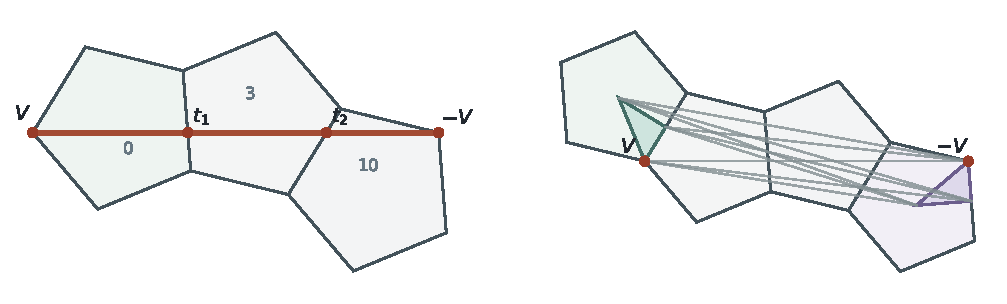
\includegraphics[width=.83\linewidth]{figures/dodeca_strips.pdf}\par
\small Left, the attaining three-face strip. Right, the two chamber triangles and their nine legal corner-to-corner routes in the four-face strip.
\end{center}
Reversing this family of paths and applying central inversion gives another strip from $C$ to $-C$, whose corner matrix is $M^{\mathsf T}$. Put $D_0^2=5+7\phi$. The gap table is particularly simple:
\[
 200\left(D_0^2\mathbf{1}_{3\times3}-\frac{M+M^{\mathsf T}}2\right)=
 \begin{pmatrix}
 [0,0]&[50,50]&[20,60]\\
 [50,50]&[100,50]&[70,10]\\
 [20,60]&[70,10]&[80,40]
 \end{pmatrix}.
\]
Here $\mathbf{1}_{3\times3}$ is the all-ones matrix. Each entry except the first is greater than $60$. Interpolation in the two strips bounds $d(x,y)^2$ by $D_0^2-\frac3{10}(1-\lambda_1\mu_1)$, with subscript $1$ marking the vertex corner. Equality requires both weights to equal one. The folding lemma preserves vertex type. The four-edge bound for the remaining vertices now gives exactly ten unordered extremal pairs and a unique farthest point from each vertex.
\subsection{An independent dodecahedral lower bound from a scalar function}

Here is a direct witness that every surface path from the chosen vertex
to its antipode has length at least $\sqrt{5+7\phi}$, where
$\phi=(1+\sqrt5)/2$. Use the faces and the two vertex labels $0,7$ of
the dodecahedral certificate. For each terminal face $F$, take all
strips of one through four distinct faces starting on any face incident
to $0$ and ending on $F$. Each strip places the source at a planar
point $s$ relative to a common chart for $F$. Put
\[
 H_F(x)=\min_s |x-s|.
\]
Every term is $1$-Lipschitz. We only need the strips to give positions
of the sites. A segment from $x$ to a site need not lift through its
strip for the Lipschitz assertion to hold.

Here are the arithmetic details for gluing these functions.
Along an oriented unit edge $ab$, write
$x=(1-t)a+tb$. A site with squared distances $r,s$ to the two ends
contributes
\[
 |x-\text{site}|^2=(1-t)r+ts-t(1-t).
\]
Discard duplicate rows $(r,s)$ and every row dominated at both ends by
another row. The two incident faces give identical surviving rows on
each of the thirty edges. The full table follows, up to reversing
the orientation. In this table $[m,n]=m+n\phi$.
\[
\begin{array}{r|l}
\text{edges}&\text{surviving rows}\\ \hline
3&(0,1)\\
6&(1,[1,1])\\
3&([1,1],[1,1])\\
6&([1,1],[3,2])\\
3&([2,3],[3,2]),\quad([3,2],[2,3])\\
6&([2,3],[3,4]),\quad([3,2],[4,4])\\
3&([3,4],[5,7])
\end{array}
\]
For a precise way to reproduce the table, start with each of the three
source faces and develop each allowed strip by the unit-edge rotation
in the face table algorithm. Record the five squared distances from
the source image to the corners of the terminal face. Remove duplicate
five-tuples. In face-label order the twelve list lengths are
$7,7,7,15,12,12,15,20,15,12,20,20$. For each edge, project each
incident list to its two endpoint columns and discard dominated rows.
The accompanying \texttt{dodeca\_calibration.py} performs precisely
these bounded ring operations and comparisons.

The identical edge formulas glue the $H_F$ to a surface function $H$
whose change along a path is bounded by its length. The squared
values at $0$ and $7$ are $0$ and $5+7\phi$. This proves the lower
bound without needing to classify shortest paths.

\section{Continuous paths and their finite certificates}\label{sec:continuity}
A continuous curve can visit a face infinitely often. A real endpoint on a mirror can be arbitrarily hard to distinguish from nearby endpoints on either side. Both issues admit finite estimates.

\paragraph{A short bridge between nearby samples.}
Use a supporting affine form $s_G\ge0$ for every face $G$, zero on $G$, scaled so its linear part has norm at most one. Choose a positive rational $\sigma$ smaller than every strictly positive vertex slack $s_G(v)$. This is finite algebraic data. For example, bound a positive slack below by rationalizing or isolating the finitely many fixed radicals in its expression. Let $b$ be an upper bound on face diameters (two suffices here). If $p\in F$, $q\in G$ and $|p-q|\le\eta<\sigma$, then $s_G(p)\le\eta$. Express $p$ as a convex combination of vertices of $F$. The total weight outside $G$ is at most $\eta/\sigma$. There must be a common vertex. Move all outside weight to a fixed such vertex. The result $r\in F\cap G$ satisfies $|p-r|\le b\eta/\sigma$. The chords $pr,rq$ form a surface bridge of length at most $(1+2b/\sigma)\eta$. A face-center weight can be distributed equally among the vertices.

For these four models one can take $b=2$, $\sigma=1/4$ throughout. For a tetrahedral or octahedral face take its outward sign normal divided by two, whose norm is $\sqrt3/2$; the positive vertex slack is $1/\sqrt2$. For the icosahedron use the unscaled coordinates $w=2p$ and the normal $n=(2\phi-2,0,-2\phi)$. The support value is $2+2\phi$ in $w$-coordinates, and its positive slacks there are $4,4\phi,4+4\phi$. The physical form with linear part $n/4$ has slacks divided by eight and $\|n/4\|=\sqrt{12}/4$. For face zero of the dodecahedron in the unscaled coordinates $w=2p/\phi$, take $n=(2-2\phi,2\phi-4,0)$. The support value is $2$, and the positive slacks there are $8-4\phi,4\phi-4,4$. In physical coordinates the linear part $n/4$ has squared norm $(28-16\phi)/16<1$ and the slacks are multiplied by $\phi/8$. The smallest is $(\phi-1)/2>1/4$. Substitution of the vertex lists verifies these finite tables. Face transitivity transfers them to the other faces.

\paragraph{Compressing a path with arbitrarily many crossings.}
Write $f$ for the number of faces. Sample a continuous curve at a mesh on which consecutive samples differ by at most $\delta$. Approximate each sample to ambient tolerance $\delta$ by a tagged surface point, retaining exact given endpoints when available. Consecutive tagged points differ by at most $3\delta$. Start at the first tag. Jump to the \emph{last} index with the same face tag, join the two tagged points by a chord, and bridge to the next tagged point by the preceding construction. Repeat from that next index. No finished face tag reappears, so at most $f$ chords and $f$ bridges are used. The sum of the chords is at most the sum of the original ambient sample increments plus $2f\delta$, by the triangle inequality on disjoint index intervals. The resulting surface polygonal path has length at most
\[
  \sum_i|\gamma(t_{i+1})-\gamma(t_i)|
    + f\,[2+3(1+2b/\sigma)]\delta,\qquad 3\delta<\sigma .
\]
The explicit choices give the error $53f\delta$. Taking $\delta=2^{-(k+11)}$ makes it less than $2^{-k}$ for $f\le20$. The sampled sum is at most the length of the original curve. Since $\delta$ is arbitrary, finite-path lower bounds hold for all rectifiable continuous curves. This proves also the asserted pathwise bound for a scalar function that is $1$-Lipschitz on convex pieces and agrees at their boundaries: split each face chord at its finitely many piece boundaries and sum the estimates. Recover exact endpoints by a short bridge if they were approximated. In the first-order interpretation a modulus supplies the mesh, and the tags belong to the input approximants.

\paragraph{Computing the intrinsic distance at prescribed precision.}
For exact tagged algebraic endpoints enumerate all lists of distinct faces whose first and last faces contain the given endpoints and whose consecutive intersections are nonempty. Include a single common face. For every shared edge allow crossings at the $2^m+1$ equally spaced grid points, and for a shared vertex allow that vertex alone. Join successive choices by face chords. Minimize the sum of their lengths rounded \emph{up} to multiples of $2^{-m}$. Call the result $U_m$. These candidates are genuine surface paths. Conversely, shorten any finite path by removing repeated faces via chords, then round its at most $f-1$ crossings to the grid on the shared intersection. This changes its length by at most $2(f-1)2^{-m}$ for unit edges. Upward length rounding contributes at most $f2^{-m}$. The two path arguments give
\[
 d\le U_m\le d+3f\,2^{-m}.
\]
Changing the endpoints by surface distances $\epsilon_x,\epsilon_y$ changes $d$ by at most $\epsilon_x+\epsilon_y$. For ambient approximations use the short-bridge estimate. A prescribed dyadic accuracy thus determines one finite search. The number of candidates is at most $\sum_{r=1}^f f^r(2^m+1)^{r-1}$, including illegal lists rejected by the checker. This algorithm defines the distance as a regular Cauchy name. At every extremal pair the proofs give a specific path attaining the distance.

\section{Arithmetizing the proof in iPRA}
Use intuitionistic first-order natural-number arithmetic with primitive recursive function symbols, their defining equations and quantifier-free induction, as in ProveIt. A statement about a real object denotes a family of bounds on finite inputs and demanded precisions. A path supplied by primitive recursive sample and modulus functions gives a schema, one instance for each choice of functions. The geometric interpretation applies externally to ordinary continuous paths with their moduli. First-order iPRA has no variable ranging over all real-valued functions.

\paragraph{Data types and exact comparisons.}
Encode signed integers by differences of naturals, rationals by a signed numerator and positive denominator, and finite lists by primitive recursive pairing and length. A solid is a fixed record of vertex coordinates, oriented face cycles and flag triples. A mesh point has a flag index and nonnegative barycentric numerators $a_0,a_1,a_2$ with positive sum $A$, meaning $\sum_i a_i C_i/A$. Weights with sum $2^m$ give a mesh: round down two weights and give the remainder to the third. The ambient error is at most $2b\,2^{-m}$. Finer meshes represent general endpoints without deciding their exact face. Interior waypoints and seams may use exact algebraic coordinates. A path code records its face list and endpoints of each segment. Test incidence with plane equations and polygon halfspaces, and equality of the two physical copies of each seam point.

Use a fixed tower of rational arithmetic and positive square roots for the model constants, for example $\sqrt2,\sqrt3,\sqrt5,\sqrt{10+2\sqrt5}$. Mirror reflections have the formula $p\mapsto p-2(n\cdot p)n/(n\cdot n)$. For pentagons the smaller ring $\mathbb Z[z]$ suffices for developed vertices and hinges, with $\operatorname{Re}(z)=(\sqrt5-1)/4$ and $\operatorname{Im}(z)=\sqrt{10+2\sqrt5}/4$. To test the sign of $a+b\sqrt r$ at a quadratic level with $r>0$, compare the signs of $a,b$ first. For opposite signs compare $a^2$ and $b^2r$ at the previous level. Represent general quotients by numerator and nonzero denominator, carrying its sign and cross-multiplying. The recursion depth of these comparisons is fixed. For a squared segment length $s$, its dyadic square-root floor is the largest integer $j$ with $j^2\le2^{2m}s$. For face chords $j\le2^{m+1}$. For a developed strip take a bound from its fixed number of faces and their diameters. The ceiling uses one further unit exactly when needed. A long sum of segment lengths needs only dyadic sums and explicit errors.

\paragraph{Object-language assertions.}
For a fixed solid $S$, a claimed pair $w,w^*$ and the positive radical $D_S$ on page one, a purely numerical specification at exact tagged endpoints is
\begin{align*}
 &\forall p,q,k\quad \mathrm{Point}_S(p)\land\mathrm{Point}_S(q)
     \ \Longrightarrow\ U_{k+c}(p,q)\le D_S+2^{-k},\\
 &\forall P,k\quad \mathrm{Path}_S(P,w,w^*)
     \ \Longrightarrow\ \sum_{e\in P}2^{-k}\lceil 2^k|e|\rceil\ge D_S .
\end{align*}
One may take $c=6$ simultaneously for the four solids, since $2^6\ge3f$. Clear positive denominators and square after checking signs to compare to $D_S$. The lower test accepts coded algebraic facewise paths of arbitrary finite length. A fixed witness strip and the mesh estimate give equality of distance names. For the upper test the inequalities give routes whose best length is at most $D_S$; rounding their crossings gives the displayed finite bound. One can compare the two resulting dyadic costs, so route selection on a real-order tie costs at most its rounding tolerance. For Cauchy input add the two explicitly controlled endpoint errors and shift the precision index. Optimal coordinates are fixed algebraic points.

\paragraph{Constructive equality cases.}
For the icosahedron and dodecahedron the gaps bound $1-\lambda_1\mu_1$. Since both weights lie in $[0,1]$, each endpoint's weight outside its vertex corner is bounded by that deficit. For the octahedron, if $d^2$ is within $\epsilon$ of $3$, each sum $\sum_{i<j}a_i a_j$ is at most $\epsilon$. Choose a largest coordinate on a finite approximant, at least $1/3$. The other coordinates sum to at most $3\epsilon$. In all three cases both endpoints are close to vertices, and nonantipodal vertices have the explicit strict upper bounds given above.

For the tetrahedron, divide each nearest-vertex quadrilateral by the diagonal joining its lattice vertex to the large triangle center $h'$. If the barycentric weight on $h'$ is $t$, convexity gives $\delta^2\le (1-t)+4t/3$. Thus $\delta^2\ge4/3-\epsilon$ places the point within $6\epsilon$ of $h'$, as the triangle diameter is at most two. Apply this to both $u+v$ and $u-v$. Their two center residues are within $6\epsilon$ of signed translates of $h$. Adding and subtracting identifies one endpoint within $6\epsilon$ of a lattice vertex and the other within $6\epsilon$ of its opposite-face center: equal signs give $v$ near a lattice vertex and $u$ near that vertex plus or minus $h$ modulo $2L$, and opposite signs reverse the roles. Folding is nonexpansive. This leaves a finite list of isolated candidate pairs in every case. Choose one precision at which neighborhoods of distinct candidates are disjoint, and keep the two approximation errors smaller than a quarter of that separation. All finer approximations must select the same unordered pair. Thus equality for names gives membership in the finite list without an exact real sign test on a mirror.

\paragraph{Permitted inductions.}
A finite fold, gallery, list minimum or bounded sign check has a primitive recursive trace and Boolean invariants. In path compression the index increases and the used-face bit mask grows. In a strip search the unused-face count decreases. A universal over indices below the loop counter is a bounded Boolean conjunction. Apply quantifier-free induction to the trace and its invariant. Rational triangle and Jensen inequalities follow after clearing denominators from nonnegative squares: Cauchy--Schwarz uses $\sum_{i<j}(u_i v_j-u_j v_i)^2$, and the variance identity subtracts $\sum_{i<j}\lambda_i\lambda_j\|u_i-u_j\|^2$. Inequalities involving square roots of segment norms may be checked on dyadic enclosures to arbitrary precision, allowing their rounding errors per segment. The compression argument bounds this count independently of the number of original samples. No compactness axiom selects an extremizer.

\section{Lean verification and formalization roadmap}
The supplied Lean sources were checked with Lean 4.32.0. Two kinds of theorem are included.
\begin{itemize}
\item \texttt{SmallCertificates.lean} checks the tetrahedral hole and the octahedral corner and permutation tables. \texttt{Icosahedron.lean} checks the two-strip matrix and the calibration tile measurements.
\item \texttt{DodecaLower.lean} enumerates the fifty strips by kernel reduction, checks the minimum multiplicity, the attaining hinge identities, and the four-edge neighborhood. \texttt{DodecaUpper.lean} constructs the four-face strip, checks all 27 intersections and the transposed gap matrix. These four files use core Lean and exact integer computation.
\item \texttt{IntrinsicIPRA.lean} and \texttt{IcosahedronIPRA.lean} construct actual derivations in ProveIt's embedded theory, of type $\Gamma\vdash_{\rm PRAAx}\varphi$. Their \texttt{octMinimum} and \texttt{icoMinimum} prove the strip-minimum bounds for arbitrary natural barycentric masses after clearing denominators. Other theorems derive a two-weight variance identity and the coordinate formula and multiplicativity of the cyclotomic squared norm. The Lean metatheory of this provider uses quotient soundness, propositional extensionality and classical choice. The object proofs use the iPRA axioms.
\item \texttt{TetrahedronIPRA.lean} derives the upper bound on a Voronoi triangle and the lower bound for every signed lattice translate at the hole. \texttt{DodecahedronIPRA.lean} derives the weighted gap bound, including the term $\frac3{10}(1-\lambda_1\mu_1)$, for the matrix as a function of a rational parameter at least one. Substitution of arbitrarily accurate rational approximants to $\phi$ gives the stated numerical interpretation.
\end{itemize}
The remaining Lean work is the geometric interpretation of these finite objects and assembly of the full object-language diameter theorems. A dependency order follows.
\begin{enumerate}
\item Build PR codes for ordered algebraic arithmetic, support forms, binary interval costs and tagged cells. Use the provider's \texttt{Core/Pairing}, \texttt{Core/Order}, \texttt{Core/Division} and bounded search modules. Prove the sign and rounding contracts one quadratic level at a time. Give realizations of the face tables, with both labelings of each shared edge. The exact dodecahedral support-plane checks are in \texttt{dodeca\_model.py}.
\item Define the predicate on facewise paths specified above. Derive chord replacement, gluing, the short bridge and rounding. Prove the precision bound on the enumerated minimum by pushing each crossing onto an edge mesh and bounding its two adjoining length changes. This connects a sample/modulus instance to the lower test.
\item Encode chamber wall reflections, the finite gallery fold, and interpolation on hinges. Invariants are the unresolved wall signs, membership of each crossing in its hinge, and the running bound on path length. Use norm identities and variance to compile the average bounds. For the tetrahedron encode lifts in a bounded fundamental parallelogram and enumerate shifts satisfying the quadratic bound.
\item Translate each fixed Boolean certificate as a closed PR term. Derive what a successful return implies about the geometry using Steps 1--3. ProveIt's \texttt{eval\_closed} in \texttt{Core/Evaluation} derives the corresponding numeral computation in the object theory. Combine with the attaining route, strict gaps and isolation argument to close the universal statements. The sampling theorem and this last assembly are provided here as mathematical proofs.
\end{enumerate}
\paragraph{Sources.}
The two attached cuboid reports supply the problem and the interpretation of surface distance. For the farthest-point map at arbitrary starting points, see J. Rouyer, \emph{Antipodes sur un t\'etraèdre r\'egulier}, J. Geom. 77 (2003), 152--170, and R. E. Schwartz's papers on the \href{https://arxiv.org/abs/2004.11852}{regular octahedron} and the \href{https://arxiv.org/abs/2104.02567}{regular dodecahedron}. The diameter calculations and certificates used here appear in the preceding sections. The object-theory implementation targets the \href{https://github.com/VladimirReshetnikov/ProveIt/tree/09fe17194da14cdd100947737952e44100bb71b8/Logic/PrimitiveRecursiveArithmetic}{ProveIt iPRA development}, revision \texttt{09fe17194d}.

\end{document}
